\documentclass{ctexart}

\usepackage{graphicx}

\usepackage{subfigure}

\usepackage{amsmath}

\usepackage{amsthm}
\newtheorem{property}{性质}

\usepackage{amssymb}

\usepackage{ulem}

\usepackage{url}

\usepackage{tikz}
\usetikzlibrary{calc,positioning,graphs,shapes,quotes,arrows}
\usepackage{ctex}
\usepackage{pgfplots}
\pgfplotsset{width=5cm,compat=1.9}

\usepackage{hyperref}
\hypersetup{hidelinks,
			colorlinks=true,
			allcolors=blue,
			pdfstartview=Fit,
			breaklinks=true}

\usepackage{geometry}
\geometry{left=2cm,right=2cm}

\title{一维非线性方程求根算法}

\author{赵天健 \\ 信息与计算科学\quad 3210101830}

\begin{document}

\maketitle

\begin{abstract}
本文对一维非线性方程求根问题, 即求解$f(x) = 0$问题的一些算法进行讨论. 这些算法主要为迭代算法( 如Newton法, 二分法等 ), 本文将逐一介绍这些算法, 并通过数学理论上的证明以及同一算例不同算法的表现来比较它们收敛速度的差异. 

\end{abstract}

\section{引言}
很久以来, 解方程都是数学家们非常关注的问题. 而解方程最基本的就是解一元方程的问题. 不过, 非线性的一元方程求解并不容易, 就算对于多项式来说也是如此. 根据Abel-Ruffini定理, 对于多项式方程$p(x) = 0$来说, 若$\deg{p} \ge 5$, 那么其没有求根公式, 而一些非多项式方程的解析解就更加难求了. 但是, 很多时候我们仍然希望在某个区间$[l, r]$内找到方程$f(x) = 0$的解, 哪怕是数值上的近似解. 为了解决这个问题, 许多迭代算法应运而生.

\section{一些求根算法的介绍}
\subsection{二分法}
这是一个朴素的想法, 后人也对此算法进行过改进( 如Brent法 ). 不过在此仅介绍此算法.
\subsubsection{数学理论}
设$f(x)$是连续函数, 现有区间$[a, b]$, 且$f(a)f(b) < 0$, 那么取区间中点$c = \frac{a+b}{2}$, 则$[a, c], [b, c]$必有至少一个区间存在$f(x)$的根. 而由于连续函数的介值定理, 则函数值与$f(c)$符号相异的端点与$c$构成的区间内必然存在根.
\subsubsection{算法流程}
\begin{figure}[htb]
\centering
\begin{tikzpicture}[node distance=10pt, hv path/.style = {to path={-| (\tikztotarget) \tikztonodes}}]
\node[draw, rounded corners]						 (sstart)   {Start};
\node[draw, rounded corners, below=of sstart]		 (start)    {给定$f$和区间$[a, b]$};
\node[draw, diamond, aspect=2, below=of start]		 (choice 1) {$b - a < eps$};
\node[draw, below=of choice 1]                       (step 1)   {计算$[a, b]$中点$c$};
\node[draw, below=of step 1]                         (step 2)   {计算$f(c)$};
\node[draw, diamond, aspect=2, below=of step 2]      (choice 2) {$f(a)f(c) < 0$};
\node[draw, rounded corners, right=20pt of choice 1] (end)      {End};
\coordinate[right=10pt of end] 						 (px);
\coordinate[left=30pt of choice 1]					 (py);

\graph{
	(start) -> (choice 1) ->["No"left] (step 1) -> (step 2) -> (choice 2);
	(choice 1) -> ["Yes"](end);
};
\draw[->] (sstart) -- (start);
\draw[rounded corners] (choice 2) -- node[above, near start] {Yes} (choice 2-|px) -> (px);
\draw[->, rounded corners] (px) -- node[above, very near end] {$[a,c]$} (px|-start) -> (start);
\draw[rounded corners] (choice 2) -- node[above, near start] {No} (choice 2-|py) -> (py);
\draw[->, rounded corners] (py) -- node[above, very near end] {$[c,b]$} (py|-start) -> (start);
\end{tikzpicture}
\caption{二分法流程图}
\label{fig:bisection}
\end{figure}

\subsubsection{收敛速度}
由上面讨论可以看出, 每迭代一次, 误差减半, 所以此算法以$R=\frac{1}{2}$的速度线性收敛.

\subsection{Newton法}
Newton法, 又称Newton-Raphson法, 是另一种找根的算法. 
\subsubsection{数学理论}
对于导函数$f'$存在的$f(x)$, 给定一个根附近的点$x_0$, 则由公式
$$
x_1 = x_0 - \frac{f(x_0)}{f'(x_0)}
$$
所产生的$x_1$是相较于$x_0$更好的对根的近似.
\begin{figure}[!ht]
	\centering
	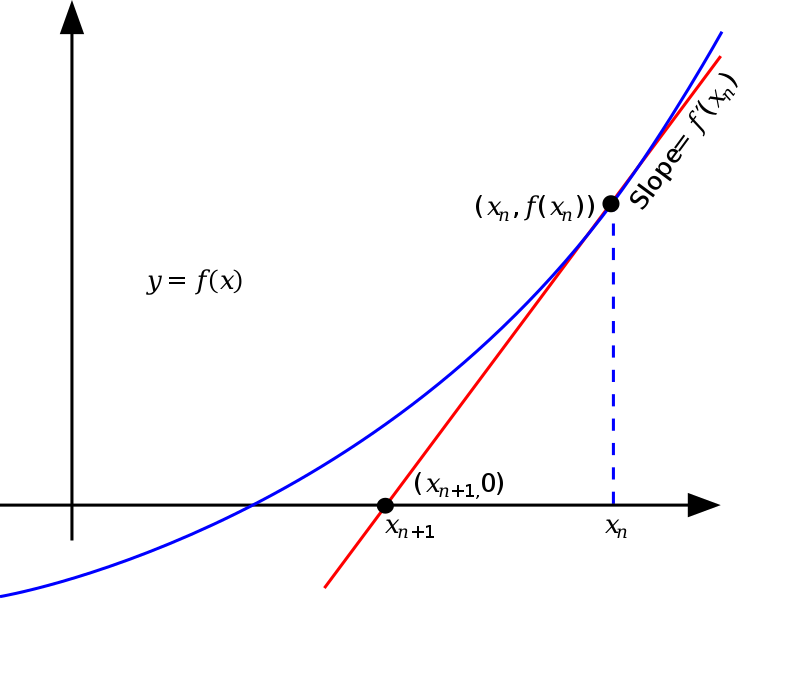
\includegraphics[width=3in]{../img/example.svg.png}
	\caption{$x_{n+1}$比$x_n$更好}
	\label{fig:wiki}
\end{figure}
\par 可以看出, 每次迭代其实是在$x_n$处将$f$看成其一阶近似, 并求解此线性方程得到新的解$x_{n+1}$.
\par 因此, 不断重复此过程, 即不断地求
\begin{equation}{section}
x_{n+1} = x_n - \frac{f(x_n)}{f'(x_n)}
\label{eq:newton}
\end{equation}
即可求得根的近似值.

\subsubsection{算法流程}
\begin{figure}[htb]
\centering
\begin{tikzpicture}[node distance=10pt, hv path/.style = {to path={-| (\tikztotarget) \tikztonodes}}]
\node[draw, rounded corners]						 (sstart)   {Start};
\node[draw, rounded corners, below=of sstart]		 (start)	{给定$f, f'$和$x_0$};
\node[draw, below=of start]							 (step 1)	{根据\ref{eq:newton}求出$x_1$};
\node[draw, diamond, aspect=2, below=of step 1]		 (choice 1) {$|x_1 - x_0| < eps$};
\node[draw, rounded corners, below=of choice 1]		 (end)		{end};
\coordinate[right=30pt of step 1]					 (px);

\graph{
	(sstart) -> (start) -> (step 1) -> (choice 1) -> ["Yes"left] (end);
};
\draw[rounded corners] (choice 1) -- node[above, near start] {No} (choice 1-|px) -> (px);
\draw[->, rounded corners] (px) -- node[above, very near end] {$x_1$} (px|-start) -> (start);

\end{tikzpicture}
\caption{Newton法流程图}
\label{fig:newton}
\end{figure}

\subsubsection{收敛速度}
可以证明, Newton方法的收敛速度是二阶的. \cite{enwiki:1095443308}

\section{通过数值算例比较上面两个算法的优劣}
由上一节关于收敛速度的讨论, 可以知道Newton法在理论上比二分法收敛的更快一些. 下面通过几个例子来比较这两个算法实际上的好坏.
\subsection{$f(x) = e^{2x}-2$}
不难知道$f(x) = 0$的解为$\frac{ln 2}{2} \approx 0.3465736$.
\par \textbf{二分法:}设置初始区间为$[0, 1], eps = 10^{-5}$, 则此算法表现如图\ref{fig:bis_exp}( 每次迭代的根为区间中点 ).
\begin{figure}[htb]
\centering
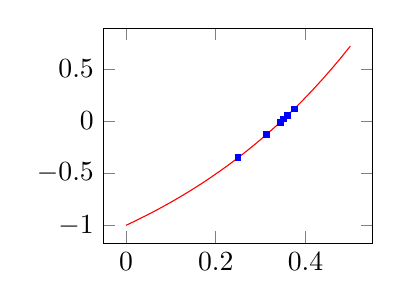
\begin{tikzpicture}
\begin{axis}
\addplot[domain=0:0.5, color=red]{exp(2 * x) - 2};
\addplot[only marks, mark=square*, color=blue, mark size=1pt]
coordinates{(0.25, -0.351278)(0.375, 0.117000)(0.3125, -0.131754)(0.34375, -0.011262)(0.359375, 0.051866)(0.351563, 0.020057)};
\end{axis}
\end{tikzpicture}
\caption{二分法}
\label{fig:bis_exp}
\end{figure}
\par 二分法迭代19次后达到目标精度.

\par \textbf{Newton法:}设置初始点$x_0 = 0, eps = 10^{-5}$, 则此算法表现如图\ref{fig:new_exp}.
\begin{figure}[htb]
\centering
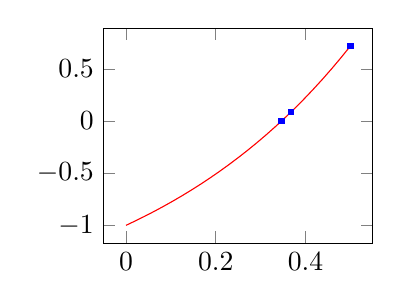
\begin{tikzpicture}
\begin{axis}
\addplot[domain=0:0.5, color=red]{exp(2 * x) - 2};
\addplot[only marks, mark=square*, color=blue, mark size=1pt]
coordinates{(0.5, 0.718282)(0.367879, 0.087063)(0.347021, 0.001790)(0.346573, 0)};
\end{axis}
\end{tikzpicture}
\caption{Newton法}
\label{fig:new_exp}
\end{figure}

\par 牛顿法迭代5次后即达到目标精度, 显著优于二分法.

\subsection{$f(x) = 8x^5 + x^4 + 9x^2 + 7x + 5$}
通过余式定理可以发现$f(x) = 0$有一解$x = -1$.
\par \textbf{二分法:}设置初始区间为$[-e, 0], eps = 10^{-5}$, 则此算法表现如图\ref{fig:bis_poly}.
\begin{figure}[htb]
\centering
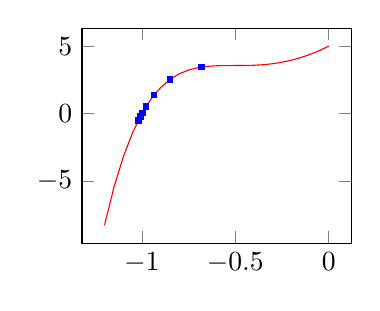
\begin{tikzpicture}
\begin{axis}
\addplot[domain=-1.2:0, color=red]{8*x^5 + x^4 + 9*x^2 + 7*x + 5};
\addplot[only marks, mark=square*, color=blue, mark size=1pt]
coordinates{(-0.679571, 3.453147)(-1.019356, -0.508801)(-0.849463, 2.530289)(-0.934409, 1.380867)(-0.976883, 0.544117)(-0.998119, 0.046796)(-1.008737, -0.223437)};
\end{axis}
\end{tikzpicture}
\caption{二分法}
\label{fig:bis_poly}
\end{figure}
\par 二分法迭代19次后达到目标精度.

\par \textbf{Newton法:}设置初始点$x_0 = 0, eps = 10^{-5}$, 则此算法表现如图\ref{fig:new_poly}.
\begin{figure}[htb]
\centering
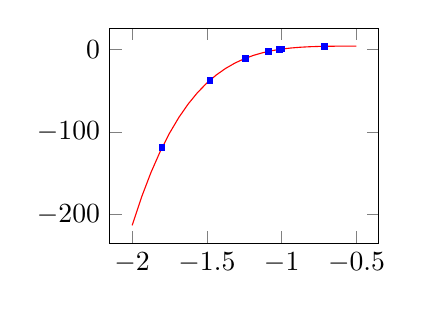
\begin{tikzpicture}
\begin{axis}
\addplot[domain=-2:-0.5, color=red]{8*x^5 + x^4 + 9*x^2 + 7*x + 5};
\addplot[only marks, mark=square*, color=blue, mark size=1pt]
coordinates{(-0.714286, 3.364669)(-1.800553, -119.313308)(-1.479526, -37.579659)(-1.243298, -11.168061)(-1.089281, -2.806756)(-1.016449, -0.429153)(-1.000672, -0.016829)};
\end{axis}
\end{tikzpicture}
\caption{Newton法}
\label{fig:new_poly}
\end{figure}
\par 牛顿法迭代9次后即达到目标精度, 显著优于二分法.

\section{结论}
可以看出, 不管是理论上还是实际例子中, Newton法在求解函数的根问题上都优于二分法, 不过其有可导的前提, 在应用上没有二分法广泛.

\bibliographystyle{plain}
\bibliography{essay}
\nocite{enwiki:1087752152}
\nocite{GSL}

\end{document}